% Options for packages loaded elsewhere
\PassOptionsToPackage{unicode}{hyperref}
\PassOptionsToPackage{hyphens}{url}
\PassOptionsToPackage{dvipsnames,svgnames,x11names}{xcolor}
%
\documentclass[
  letterpaper,
  DIV=11,
  numbers=noendperiod]{scrreprt}

\usepackage{amsmath,amssymb}
\usepackage{iftex}
\ifPDFTeX
  \usepackage[T1]{fontenc}
  \usepackage[utf8]{inputenc}
  \usepackage{textcomp} % provide euro and other symbols
\else % if luatex or xetex
  \usepackage{unicode-math}
  \defaultfontfeatures{Scale=MatchLowercase}
  \defaultfontfeatures[\rmfamily]{Ligatures=TeX,Scale=1}
\fi
\usepackage{lmodern}
\ifPDFTeX\else  
    % xetex/luatex font selection
\fi
% Use upquote if available, for straight quotes in verbatim environments
\IfFileExists{upquote.sty}{\usepackage{upquote}}{}
\IfFileExists{microtype.sty}{% use microtype if available
  \usepackage[]{microtype}
  \UseMicrotypeSet[protrusion]{basicmath} % disable protrusion for tt fonts
}{}
\makeatletter
\@ifundefined{KOMAClassName}{% if non-KOMA class
  \IfFileExists{parskip.sty}{%
    \usepackage{parskip}
  }{% else
    \setlength{\parindent}{0pt}
    \setlength{\parskip}{6pt plus 2pt minus 1pt}}
}{% if KOMA class
  \KOMAoptions{parskip=half}}
\makeatother
\usepackage{xcolor}
\setlength{\emergencystretch}{3em} % prevent overfull lines
\setcounter{secnumdepth}{5}
% Make \paragraph and \subparagraph free-standing
\ifx\paragraph\undefined\else
  \let\oldparagraph\paragraph
  \renewcommand{\paragraph}[1]{\oldparagraph{#1}\mbox{}}
\fi
\ifx\subparagraph\undefined\else
  \let\oldsubparagraph\subparagraph
  \renewcommand{\subparagraph}[1]{\oldsubparagraph{#1}\mbox{}}
\fi


\providecommand{\tightlist}{%
  \setlength{\itemsep}{0pt}\setlength{\parskip}{0pt}}\usepackage{longtable,booktabs,array}
\usepackage{calc} % for calculating minipage widths
% Correct order of tables after \paragraph or \subparagraph
\usepackage{etoolbox}
\makeatletter
\patchcmd\longtable{\par}{\if@noskipsec\mbox{}\fi\par}{}{}
\makeatother
% Allow footnotes in longtable head/foot
\IfFileExists{footnotehyper.sty}{\usepackage{footnotehyper}}{\usepackage{footnote}}
\makesavenoteenv{longtable}
\usepackage{graphicx}
\makeatletter
\def\maxwidth{\ifdim\Gin@nat@width>\linewidth\linewidth\else\Gin@nat@width\fi}
\def\maxheight{\ifdim\Gin@nat@height>\textheight\textheight\else\Gin@nat@height\fi}
\makeatother
% Scale images if necessary, so that they will not overflow the page
% margins by default, and it is still possible to overwrite the defaults
% using explicit options in \includegraphics[width, height, ...]{}
\setkeys{Gin}{width=\maxwidth,height=\maxheight,keepaspectratio}
% Set default figure placement to htbp
\makeatletter
\def\fps@figure{htbp}
\makeatother
% definitions for citeproc citations
\NewDocumentCommand\citeproctext{}{}
\NewDocumentCommand\citeproc{mm}{%
  \begingroup\def\citeproctext{#2}\cite{#1}\endgroup}
\makeatletter
 % allow citations to break across lines
 \let\@cite@ofmt\@firstofone
 % avoid brackets around text for \cite:
 \def\@biblabel#1{}
 \def\@cite#1#2{{#1\if@tempswa , #2\fi}}
\makeatother
\newlength{\cslhangindent}
\setlength{\cslhangindent}{1.5em}
\newlength{\csllabelwidth}
\setlength{\csllabelwidth}{3em}
\newenvironment{CSLReferences}[2] % #1 hanging-indent, #2 entry-spacing
 {\begin{list}{}{%
  \setlength{\itemindent}{0pt}
  \setlength{\leftmargin}{0pt}
  \setlength{\parsep}{0pt}
  % turn on hanging indent if param 1 is 1
  \ifodd #1
   \setlength{\leftmargin}{\cslhangindent}
   \setlength{\itemindent}{-1\cslhangindent}
  \fi
  % set entry spacing
  \setlength{\itemsep}{#2\baselineskip}}}
 {\end{list}}
\usepackage{calc}
\newcommand{\CSLBlock}[1]{\hfill\break\parbox[t]{\linewidth}{\strut\ignorespaces#1\strut}}
\newcommand{\CSLLeftMargin}[1]{\parbox[t]{\csllabelwidth}{\strut#1\strut}}
\newcommand{\CSLRightInline}[1]{\parbox[t]{\linewidth - \csllabelwidth}{\strut#1\strut}}
\newcommand{\CSLIndent}[1]{\hspace{\cslhangindent}#1}

\KOMAoption{captions}{tableheading}
\makeatletter
\@ifpackageloaded{bookmark}{}{\usepackage{bookmark}}
\makeatother
\makeatletter
\@ifpackageloaded{caption}{}{\usepackage{caption}}
\AtBeginDocument{%
\ifdefined\contentsname
  \renewcommand*\contentsname{Table of contents}
\else
  \newcommand\contentsname{Table of contents}
\fi
\ifdefined\listfigurename
  \renewcommand*\listfigurename{List of Figures}
\else
  \newcommand\listfigurename{List of Figures}
\fi
\ifdefined\listtablename
  \renewcommand*\listtablename{List of Tables}
\else
  \newcommand\listtablename{List of Tables}
\fi
\ifdefined\figurename
  \renewcommand*\figurename{Figure}
\else
  \newcommand\figurename{Figure}
\fi
\ifdefined\tablename
  \renewcommand*\tablename{Table}
\else
  \newcommand\tablename{Table}
\fi
}
\@ifpackageloaded{float}{}{\usepackage{float}}
\floatstyle{ruled}
\@ifundefined{c@chapter}{\newfloat{codelisting}{h}{lop}}{\newfloat{codelisting}{h}{lop}[chapter]}
\floatname{codelisting}{Listing}
\newcommand*\listoflistings{\listof{codelisting}{List of Listings}}
\makeatother
\makeatletter
\makeatother
\makeatletter
\@ifpackageloaded{caption}{}{\usepackage{caption}}
\@ifpackageloaded{subcaption}{}{\usepackage{subcaption}}
\makeatother
\ifLuaTeX
  \usepackage{selnolig}  % disable illegal ligatures
\fi
\usepackage{bookmark}

\IfFileExists{xurl.sty}{\usepackage{xurl}}{} % add URL line breaks if available
\urlstyle{same} % disable monospaced font for URLs
\hypersetup{
  colorlinks=true,
  linkcolor={blue},
  filecolor={Maroon},
  citecolor={Blue},
  urlcolor={Blue},
  pdfcreator={LaTeX via pandoc}}

\author{}
\date{}

\begin{document}

\renewcommand*\contentsname{Table of contents}
{
\hypersetup{linkcolor=}
\setcounter{tocdepth}{2}
\tableofcontents
}
\bookmarksetup{startatroot}

\chapter{Buddhi GV}\label{buddhi-gv}

\begin{center}
\includegraphics[width=0.7\textwidth,height=\textheight]{images/\%5Bremoval.ai\%5D_162b22c6-11a8-4ac1-9036-2dadecac939a-title.png}
\end{center}

The project aims to democratize access and understanding of BCI
(Brain-Computer Interfaces), particularly non-invasive EEG devices. This
website is curated as a supporting repository to a conceptual kiosk
proposed to be set up in NIMHANS Museum or other public spaces.

The main objective is to compile useful information and resources around
the theme of Brain computer interfaces to foster curiosity,
experimentation and speculation.

If you are someone who engages with BCI and non-invasive EEG devices of
any kind, your contribution to this website would be much appreciated.
The github repository can be found here.

\part{Curiosity}

\chapter{Introduction to BCI}\label{introduction-to-bci}

BCI stands for Brain Computer interfaces. BCIs are devices that let the
human brain communicate with and control external software or hardware.
It is a communication pathway between the brain's electrical activity
and an external device, in this case a computer.

BCIs are primarily of three kinds - invasive, partially invasive,
non-invasive.

\begin{figure}[H]

{\centering 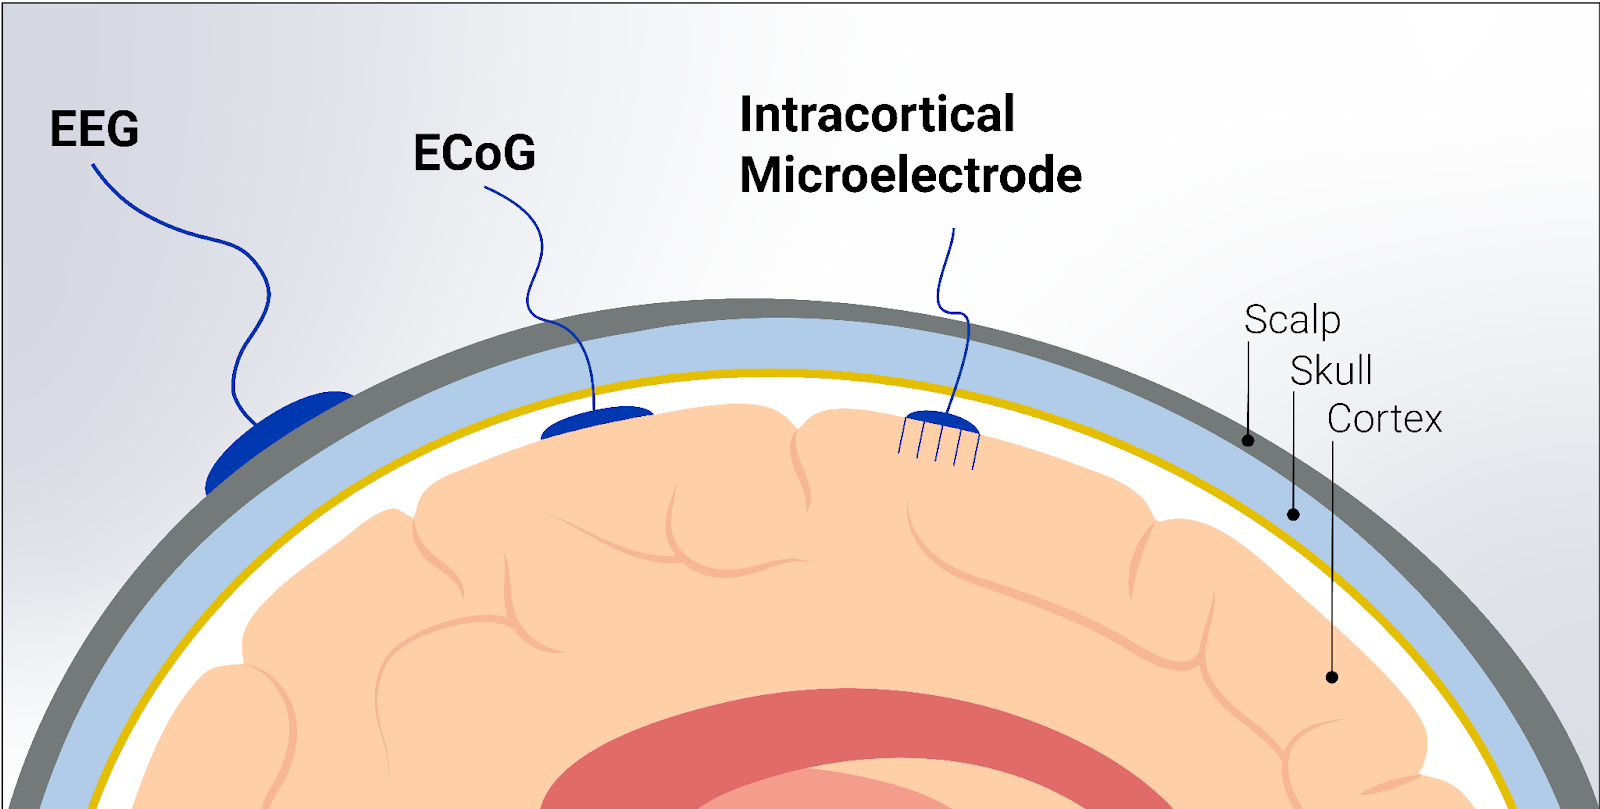
\includegraphics{images/65cd1a545634de6df4638f0e_6279ab07c6628c70c87853b8_WKwprEdZXs6z8tzbspUAF13_Kd1uMTjgOoUkj6JFHHzsvWTUbYqQ14ngYRgLn7moghtgD3BgTkdVztJxo7MyeEx3crcEsfs6pRA3GxlSooLQMma_ewcmbvapPqCwSFd0Ae59e0EebQRL1-Ql3w.png}

}

\caption{Image source:
https://www.paradromics.com/blog/enabling-connection-ii-bci-for-assistive-communication}

\end{figure}%

\subsection{Invasive BCIs}\label{invasive-bcis}

A brain computer interface is said to be invasive if it involves surgery
to implant micro electrodes under the scalp. They are implanted directly
into the grey matter of the brain and produce the highest quality
signals.

The earliest examples of invasive BCIs have been in the field of
artificial vision and motor neuroprosthetics. Direct brain implants have
been used to treat acquired blindness. One of the first scientists to
produce a working brain interface to restore sight was private
researcher William Dobelle (Kotler, n.d.) Researchers at Emroy
University in Atlanta were the first to install a brain implant strong
enough to simulate movement (Kennedy and Bakay 1998)

\subsection{Partially invasive BCI}\label{partially-invasive-bci}

These are brain computer interfaces that are implanted into the skull
but rest outside the brain and not inside the grey matter. The most
popular example of partially invasive BCI is ECoG.

ECoG stands for Electrocorticography. ECoG measures electrical activity
of the brain from beneath the skull. The earliest trials for ECoG were
done in the Washington University in St.~Louis, one of the experiments
enables a participant to play the game Space Invaders using his ECoG
implant (Lutz 2006)

\subsection{Non Invasive BCI}\label{non-invasive-bci}

These are brain computer interfaces that do not require surgery or
implants of any kind. They are predominantly EEG
(Electroencephalography) devices. These interfaces are easier to wear.
However they have poor spacial resolution and the skull dampens some
signals. Additionally EEG devices require time and effort to get useful
signals and readable electrical activity prior every session.

\chapter{Non Invasive EEG}\label{non-invasive-eeg}

Non invasive EEG refers to brain computer interfaces that use electrodes
that are placed on the scalp to record the electrical activity of the
brain. They use a method called EEG which stands for
Electroencephalography.

Voltage fluctuations measured by a bioamplifier and electrodes allow the
evaluation of normal brain activity. As the electrical activity
monitored by EEG originates in neurons in the underlying brain tissue,
the recordings made by the electrodes on the surface of the scalp vary
in accordance with their orientation and distance to the source of the
activity.

A healthy EEG ranges between the frequency of 1 and 30~Hz, and
amplitudes will vary between 20 and 100 μV.

\section{EEG Bands}\label{eeg-bands}

Based on the frequency of the electrical activity, EEG is divided into
subgroups. The different types of brain waves are

\begin{itemize}
\item
  Delta (less than 4 Hz): Delta waves are observed in the EEG signal
  when a person is asleep
\item
  Theta (4--8 Hz): Theta waves are observed when a person is sleepy or
  drowsy
\item
  Alpha (8--13 Hz): Alpha waves are observed when a person is relaxed
  where the muscles are loose but they are awake.
\item
  Beta (13--30 Hz): Beta waves are prominent when a person is alert,
  busy, active or similar states
\item
  Gamma (30--100 Hz): Gamma waves are observed when a person is trying
  to solve a problem
\end{itemize}

\begin{figure}[H]

{\centering 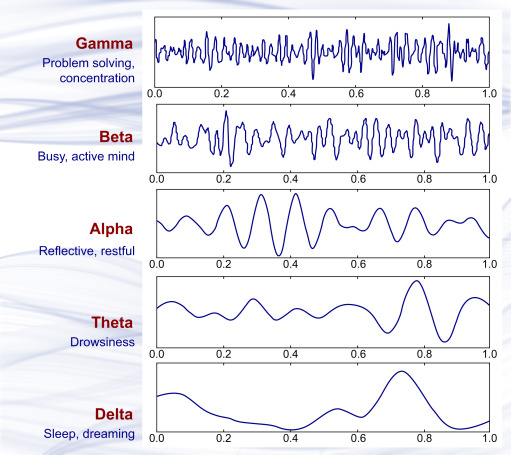
\includegraphics[width=1\textwidth,height=\textheight]{images/3-s2.0-B9780128044902000026-f02-01-9780128044902.jpg}

}

\caption{image source:
https://ars.els-cdn.com/content/image/3-s2.0-B9780128044902000026-f02-01-9780128044902.jpg}

\end{figure}%

\section{International 10-20 System}\label{international-10-20-system}

The 10-20 system is a globally accepted method to describe and apply
scalp electrodes on a person's head while recording EEG. Depending on
the number of electrodes available and the EEG band primarily being
recorded, the placement on the scalp is decided.

\begin{itemize}
\item
  Each electrode placement site has a letter to identify area of the
  brain it is reading from: pre-frontal (Fp), frontal (F), temporal (T),
  parietal (P), occipital (O), and central (C).
\item
  ``Z'' electrodes are often utilized as `grounds' or `references'. FpZ,
  Fz, Cz, Oz are zero sites and present mostly for reference/measurement
  points.
\item
  Even-numbered electrodes (2,4,6,8) refer to electrode placement on the
  right side of the head, whereas odd numbers (1,3,5,7) refer to those
  on the left
\end{itemize}

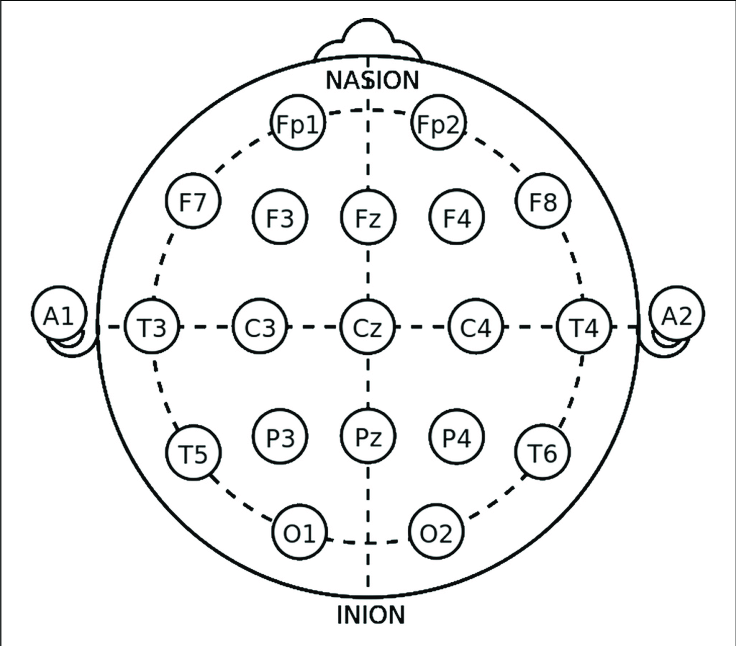
\includegraphics{images/The-10-20-International-system-of-EEG-electrode-placement.png}

\chapter{Medical applications of EEG}\label{medical-applications-of-eeg}

\section{EEG as a diagnostic tool}\label{eeg-as-a-diagnostic-tool}

EEG is the most commonly practices diagnostic procedure to confirm
epilepsy. Given the low to moderate sensitivity, a routine EEG
(typically with a duration of 20--30 minutes) can be normal in people
that have epilepsy. When an EEG shows sharp waves, spikes etc, it is
confirmatory of epilepsy in nearly all cases. It could also help in the
diagnosis of brain tumor, brain damage from head injury, brain
dysfunction etc

\begin{figure}[H]

{\centering 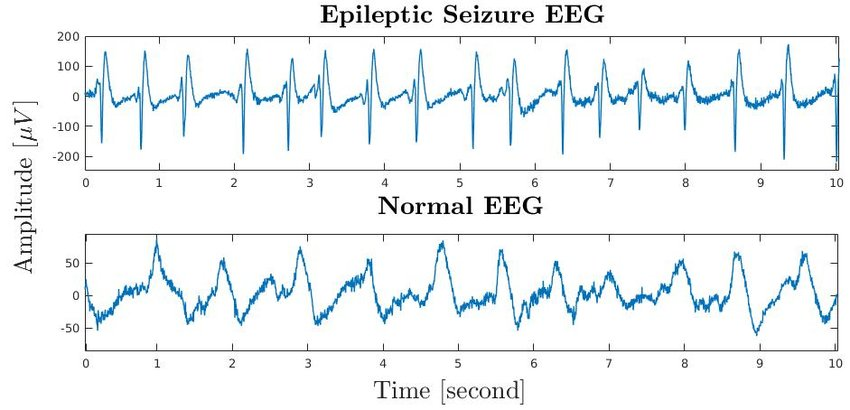
\includegraphics{images/Epileptic-Seizure-EEG-vs-Normal-EEG.jpg}

}

\caption{Image credits: Natalia Espinosa}

\end{figure}%

\section{EEG in Neurofeedback
therapy}\label{eeg-in-neurofeedback-therapy}

Neurofeedback (NFB) is a branch of biofeedback in which participants can
visualize their brain activity and try and regulate it to reach an
optimal state. Neurofeedback is a non-invasive method that assists
subjects to control their brain waves consciously. It is often done
through simple games and activities. Electroencephalography (EEG)
signals are recorded during neurofeedback and its various components
based on frequencies are extracted and visualized to create a feedback
loop.

There exist various neurofeedback treatment protocols i.e.~alpha, beta,
alpha/theta, delta, gamma, and theta, the protocol is decided based on
the patient's specific case requirements. Different EEG electrode
placements also exist i.e.~standard recording channels in the frontal,
temporal, central, and occipital lobes.

There are multiple implications of NFB therapy i.e.~treatment of
attention deficit hyperactivity disorder, anxiety, depression, epilepsy,
insomnia, drug addiction, schizophrenia, learning disabilities, dyslexia
and dyscalculia, autistic spectrum disorders and so on as well as other
applications such as pain management, and the improvement of musical and
athletic performance. (Marzbani, Marateb, and Mansourian 2016)

\url{https://www.youtube.com/watch?v=-OTTenzRqR8}

\chapter{Consumer Applications of
EEG}\label{consumer-applications-of-eeg}

Consumer grade plug and play Bluetooth EEG headsets are available across
different countries. Popular manufacturers include EMOTIV, Neurosky,
Muse, OpenBCI etc. The cost of these devices range from \$20 to \$99,000

A comprehensive list of famous BCI hardware, can be found here:

\section{EEG devices in India}\label{eeg-devices-in-india}

The market for EEG devices in India is still very nacent. Most
manufacturers do not deliver to India. Although, there are new companies
with EEG products that are gaining popularity.

\subsection{\texorpdfstring{\href{https://upsidedownlabs.tech/}{UpsideDownLabs}}{UpsideDownLabs}}\label{upsidedownlabs}

UpsideDownLabs is a company aimed at making Do-It-Yourself (DIY)
Neuroscience affordable and accessible to all so that students and
researchers can make innovative projects in Brain-Computer Interface
(BCI) and Human-Computer Interface (HCI) at ease. They mainly sell
sensors, electrodes and kits with Arduinos to experiment with.

Popular products:

\begin{itemize}
\item
  \href{https://store.upsidedownlabs.tech/product/bioamp-exg-pill/}{BIOAMP
  EXG Pill}
\item
  \href{https://store.upsidedownlabs.tech/product/diy-neuroscience-kit-pro/}{DIY
  Neuroscience Kit}
\item
  \href{https://store.upsidedownlabs.tech/product/muscle-bioamp-candy/}{Muscle
  BIOAMP candy}
\end{itemize}

\url{https://www.youtube.com/watch?v=4IGVcofhE30}

\subsection{\texorpdfstring{\href{https://nemaai.com/}{Nema
AI}}{Nema AI}}\label{nema-ai}

NEMA AI is a startup based in India that uses neuroscience and
artificial intelligence (AI) to provide solutions for education,
employability, and marketing. NEMA AI is a service provider. They
utilize Emotiv brand's 5 or 14 channel EEG headsets in a concise
5-minute session, capturing users' brain patterns. Following the scan,
users receive counseling and career guidance, elucidating effective
measures for progress and goal achievement.

\url{https://www.youtube.com/watch?v=OCL164onwvI&pp=ygUSbmVtYSBhaSBzaGFyayB0YW5r}

\subsection{\texorpdfstring{\href{https://neuphony.com/}{Neuphony}}{Neuphony}}\label{neuphony}

Neuphony empowers individuals to train and reinforce desired brain
activity through biofeedback using EEG technology. By offering real-time
data feedback, Neuphony enables users to understand and optimise their
practises and routines.

Neuphony is an Indian brand that sells EEG headsets along with their
mobile app. With real time data from the headset, one can take up
different neurofeedback and brain training sessions on their app to
imrove brain health.

\begin{itemize}
\item
  \href{https://neuphony.com/brain-wearables/eeg-headband/}{Neuphony -
  Wearable EEG headband for Brain health}
\item
  \href{https://neuphony.com/diy-neuroscience-kits/exg-synapse/}{Neuphony
  - EXG Synapse Open Source Kit}
\item
  \href{https://neuphony.com/softwares/mobile-application/}{Neuphony -
  Mobile Application}
\end{itemize}

\url{https://www.youtube.com/watch?v=qJacs2gy3Ds}

\chapter{EEG in Art and Performance}\label{eeg-in-art-and-performance}

\subsection{MindPool}\label{mindpool}

MindPool was an installation that encouraged self-reflection through
biofeedback. It collected alpha, beta, delta, and theta brainwaves to
create ripples in 48 shallow pools of water thanks. The installation is
the work of an artist called Lisa Park. (Long and Vines 2013)

\url{https://www.youtube.com/watch?v=F-r-ZGE4z_M}

\subsection{Original Ideal}\label{original-ideal}

With Original Ideal, Chasserot explores new ideas about beauty being a
function of personal identity, as opposed to the contexts of societal
standards. The first step involves capturing images of his subjects in
minimal, basic, and effortless states. Followed by digital modifica-
tions to the captured image. The participants are then hooked up to an
Emotiv EEG brain scanner, and shown 50 edited images. Those brain scans
are then analyzed for brain activity that can denote a positive
emotional reaction to understand how our brain responds to societal
standards of beauty. (Mufson 2014)

\url{https://vimeo.com/83598327}

\subsection{Interactive Brain Light}\label{interactive-brain-light}

Interactive Brain Light is artist Laura Jade's new EEG- controlled
installation, Brain Light Project is a light sculpture designed to
create a biofeedback loop of light, sound, and thought. In a process
developed by Jade, neuroscientist Peter Simpson-Young, and programmer
Sam Gentle, the installation becomes a real-time visualization of
visitors' alpha, theta, and beta brainwaves. (Laura Jade 2015)

\url{https://www.youtube.com/watch?v=-gA0U1WMUNg}

\part{Experimentation}

\chapter{Setup to record EEG from the visual
cortex}\label{setup-to-record-eeg-from-the-visual-cortex}

\section{Materials Required}\label{materials-required}

\begin{itemize}
\item
  Bio Amp EXG Pill (soldered)
\item
  Gel electrode patches
\item
  Electrode headband
\item
  Conductive gel
\item
  Arduino and connector cable
\item
  Jumper wires
\item
  Laptop
\end{itemize}

\section{Assembling the circuit}\label{assembling-the-circuit}

The BIOAMP EXG Pill is connected to an Arduino board one end using
jumper wires and to the electrodes on the other end. Connect the Arduino
to a laptop.

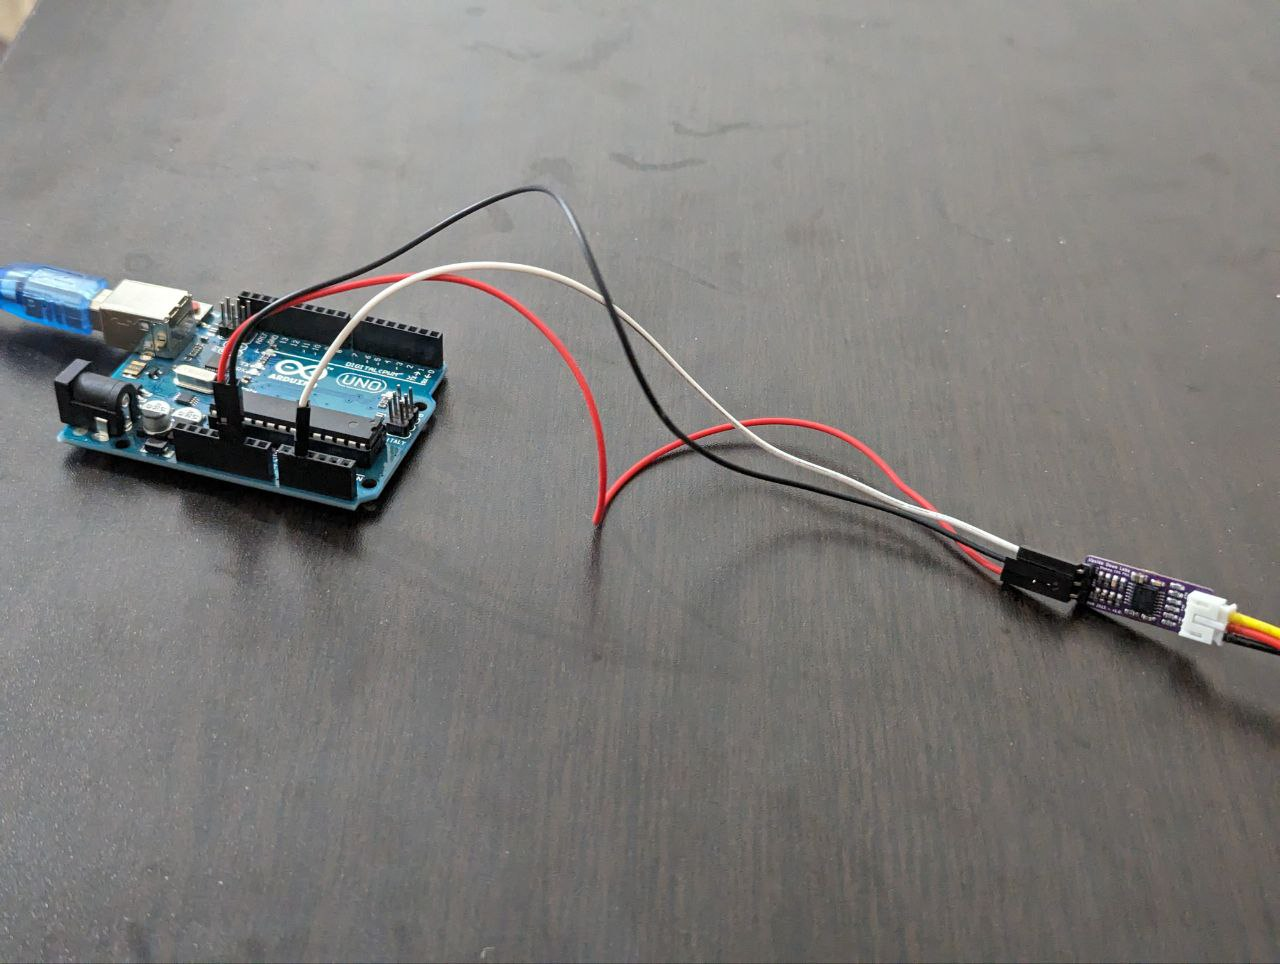
\includegraphics{images/clipboard-853366779.png}

The positive and negative wires are connected to the band and the ground
wire is connected to a gel electrode.

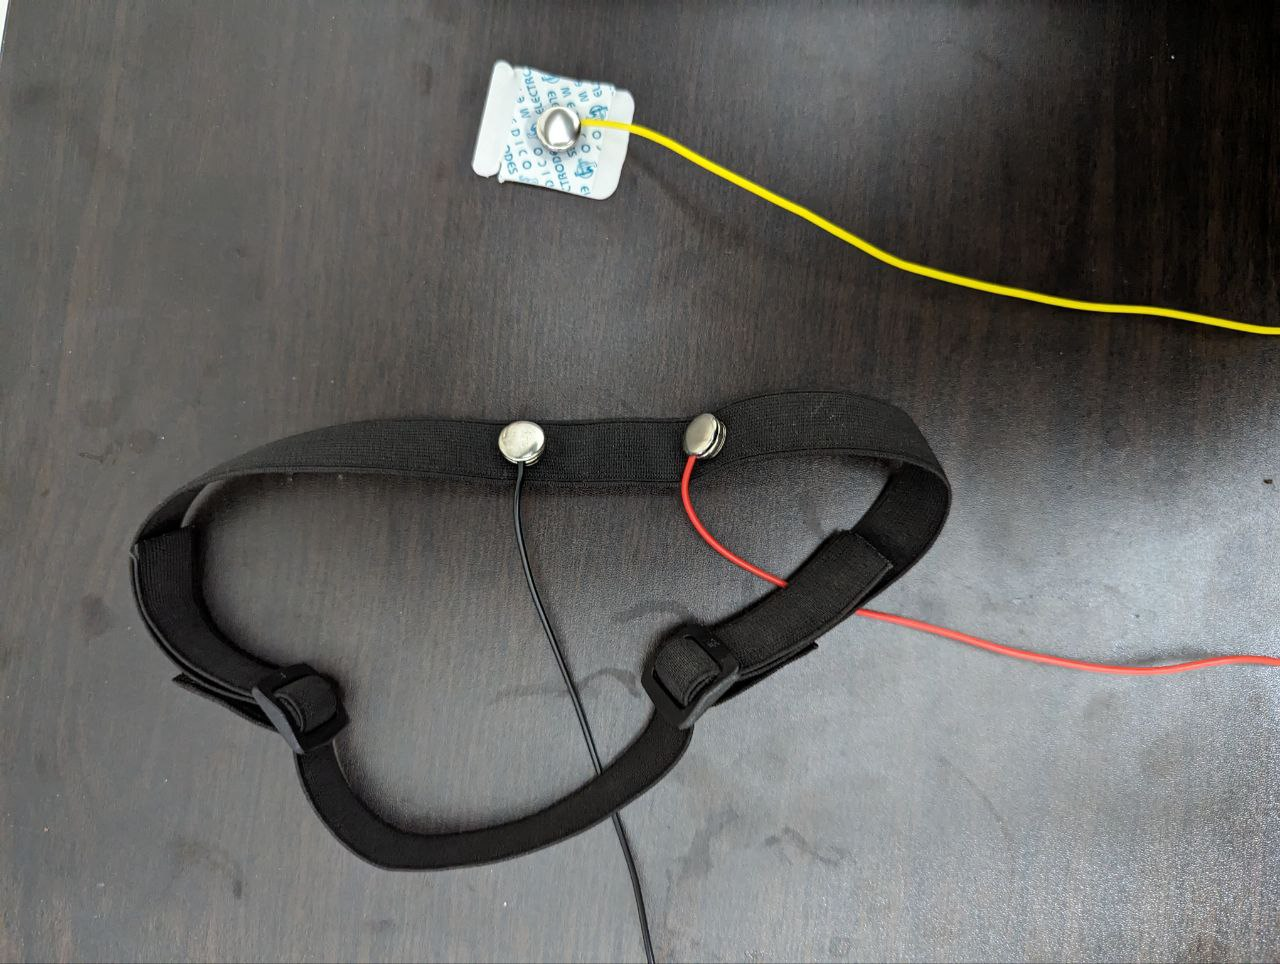
\includegraphics{images/clipboard-4134519690.png}

\section{Placing the electrodes on the
scalp}\label{placing-the-electrodes-on-the-scalp}

The band needs to be worn by the user, tightly enough so that there is
not gap between the electrodes and the scalp. The band needs to worn in
such a way that it is touching the scalp directly. Apply some conductive
gel on both electrodes to improve the signal reading.

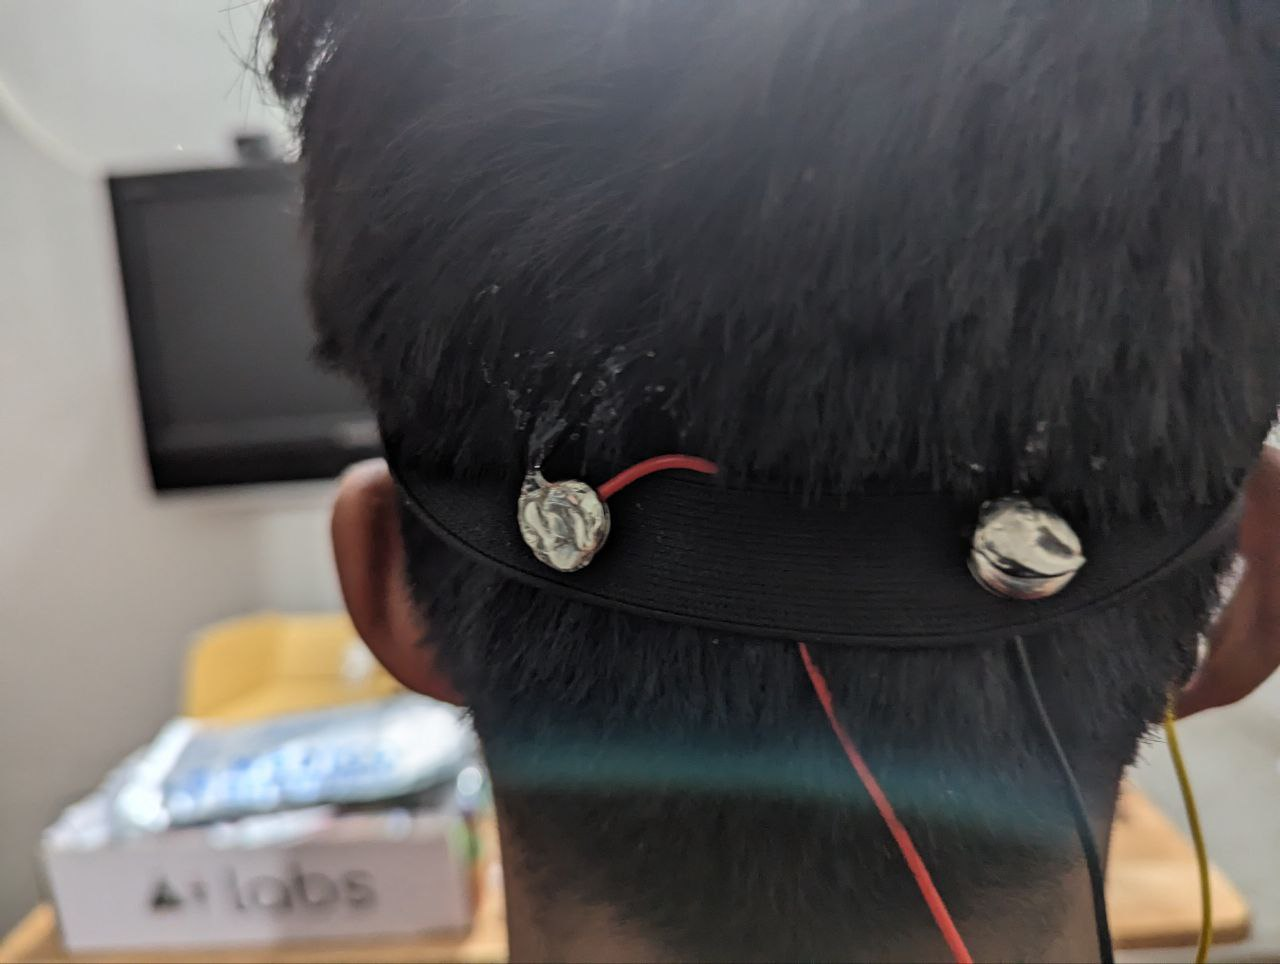
\includegraphics{images/clipboard-2783055425.png}

The placement of the positive and negative electrodes must be on the
back of the head. I have tried multiple placements, I have gotten clean
results when the electrodes are placed behind the head slightly above
the ear. Place the ground electrode with the gel electrode patch behind
the participants right ear.

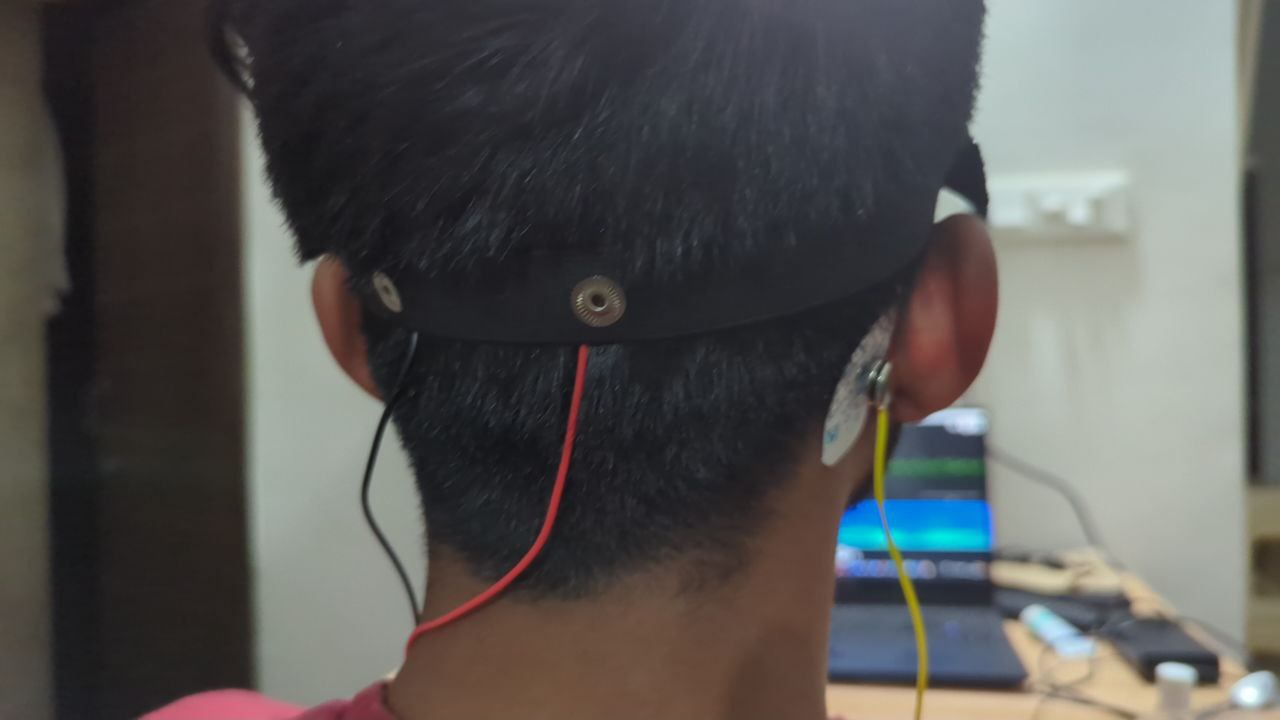
\includegraphics{images/clipboard-1512373558.png}

\section{Things that might help}\label{things-that-might-help}

\begin{itemize}
\item
  There must be no switched on electrical appliances or AC current
  devices very close to the sensor. This includes charging your laptop,
  connecting HDMI to an external monitor etc.
\item
  The users needs to sit stable and minimize movement as much as
  possible. Any movements like eyebrow movements, eye blinks etc will
  cause interference in the signal
\item
  It will take 5 to 10 minutes to get the user and the interface
  adjusted to each other. Until then feel free to try out different
  positions and placements. Feel free to add the conductive gel once
  again while readjusting the placement of the electrodes. It might take
  some trial and error to get clean readings.
\item
  Once the session is done, it is advisable for users to wash their
  hair. Wash the band and the + and - electrodes once you are done.
  Prolonged exposure to the gel might corrode the electrode.
\end{itemize}

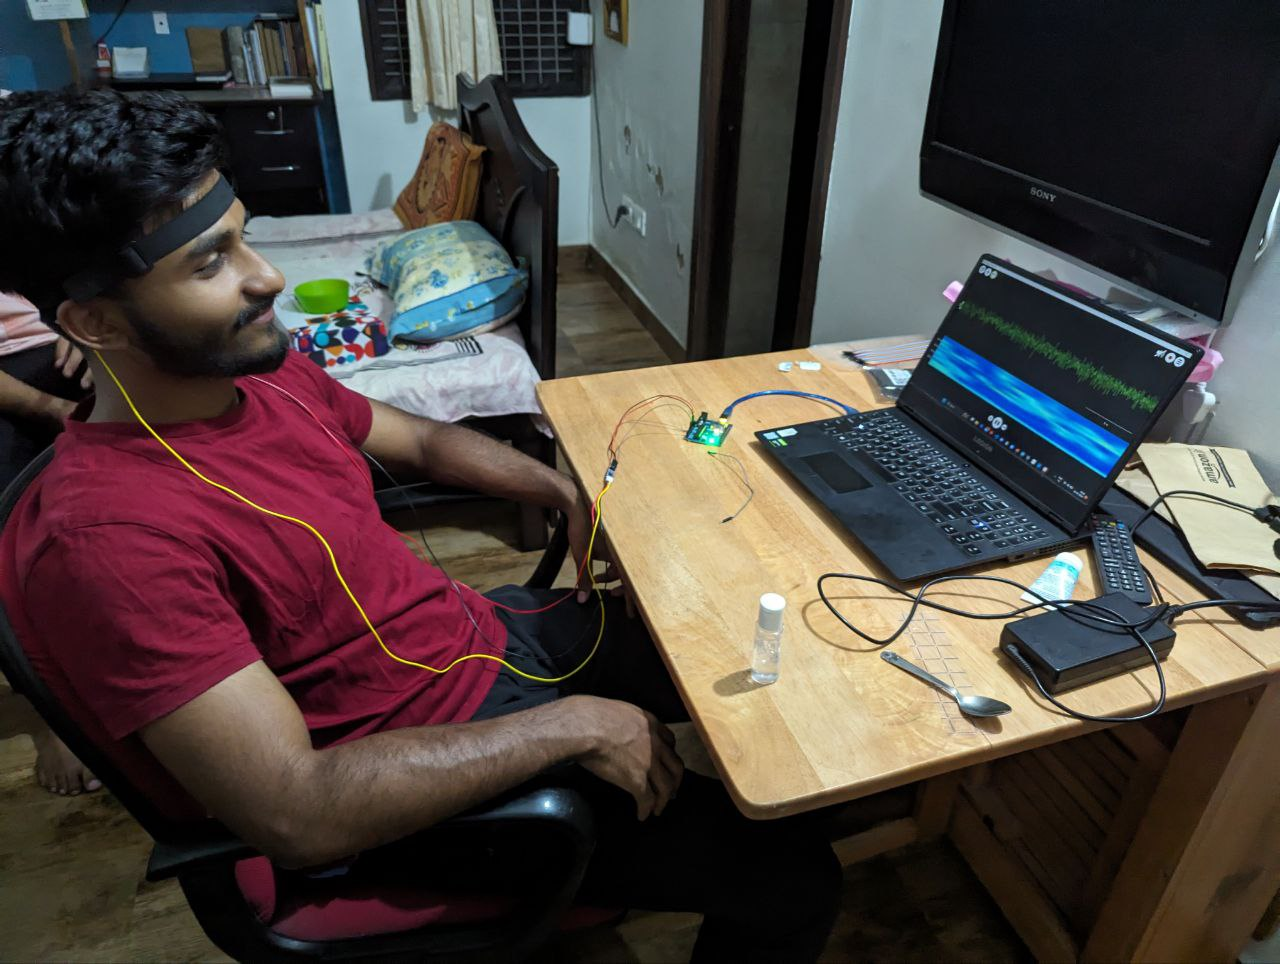
\includegraphics{images/clipboard-2267831741.png}

\chapter{Connecting the setup to the Spike Recorder
app}\label{connecting-the-setup-to-the-spike-recorder-app}

In this experiment, we will look at how to connect the BioAmp EXG Pill
and Arduino that we setup to the Spike recorder app. Spike recorder is a
tool that helps visualize bio potential signals. It also comes with
helpful tools like FFT graphs, frequency filters etc

\section{Install Backyard Brains - Spike Recorder
app}\label{install-backyard-brains---spike-recorder-app}

The first step in this process is to install the backyard brains spike
recorder app. You can find the link for the installation
\href{https://backyardbrains.com/products/spikerecorder}{here}

\begin{center}
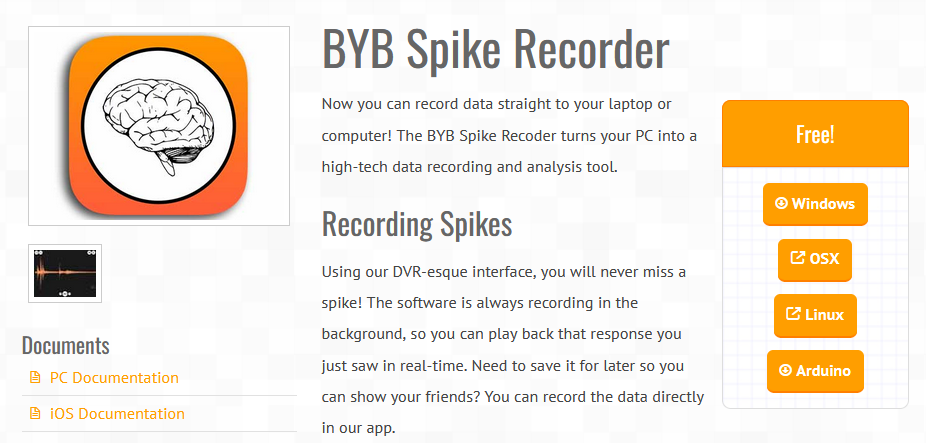
\includegraphics{images/clipboard-1284036578.png}
\end{center}

\section{Arduino script}\label{arduino-script}

Once the app is installed, you will need an Arduino script to
communicate with the app through a serial port. I used the script
provided by Backyard Brain itself. The script was written to connect
their Muscle SpikerShield product, but the same script works with the
Bio Amp EXG Pill as well.

The code for this script can be found here. Run this script and upload
it to the Arduino board. Make sure you remember the serial port the
Arduino transmits data to. In the case of my Windows laptop, it was
COM14.

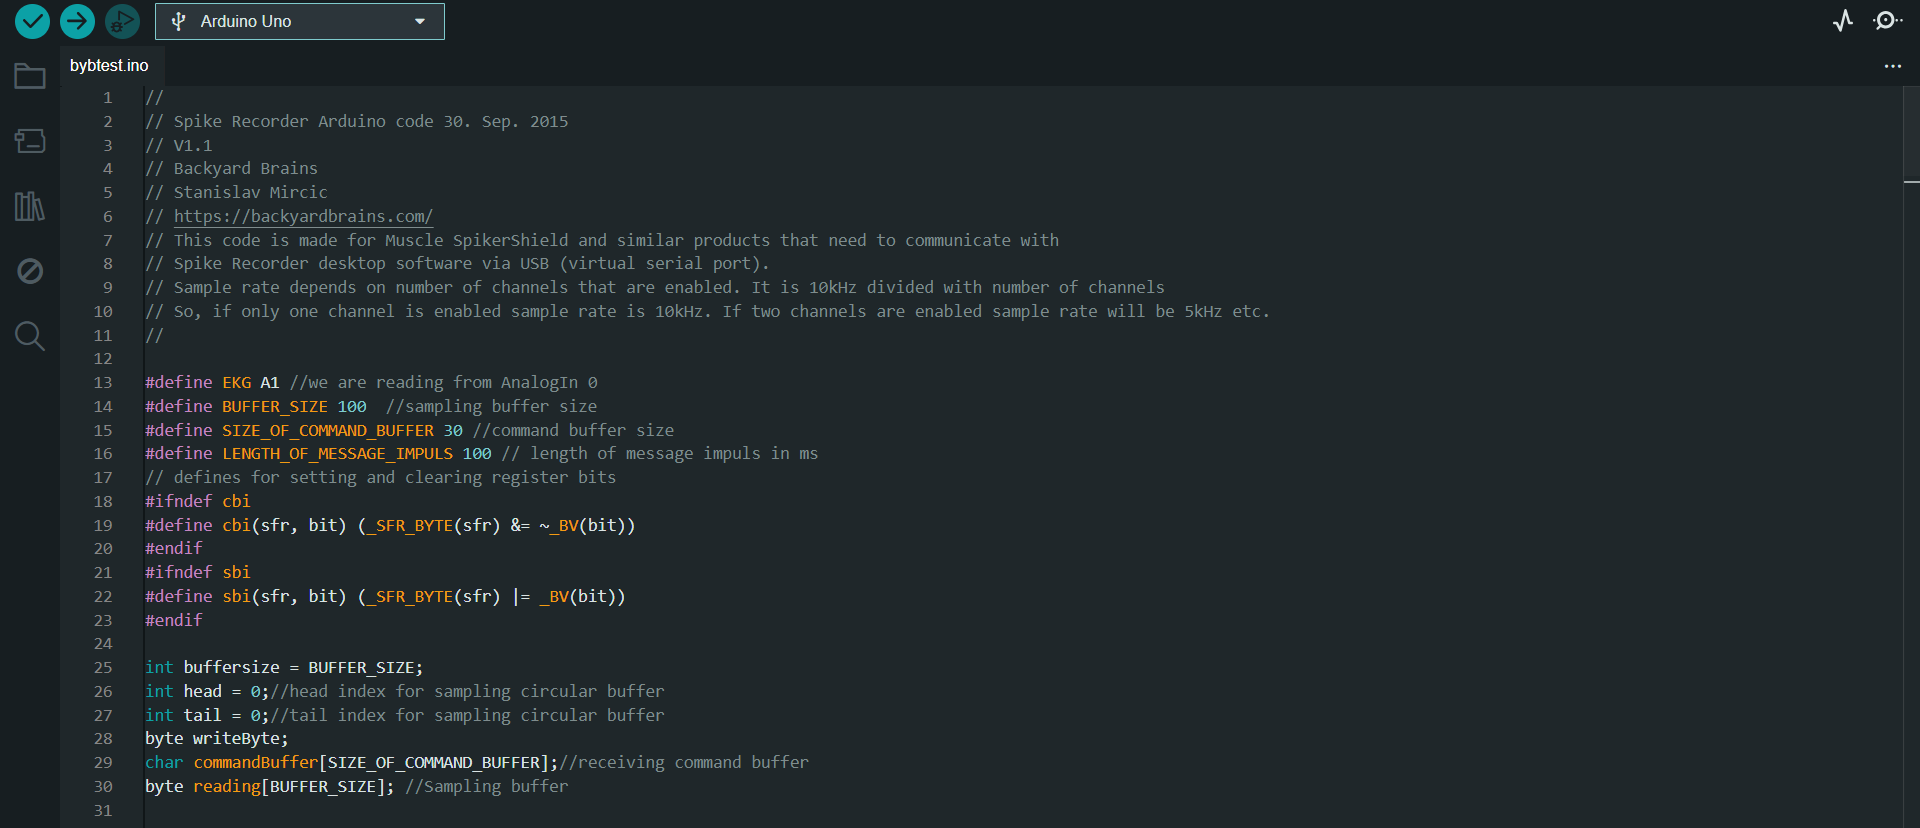
\includegraphics{images/clipboard-2071281161.png}

\section{Spike Recorder app
configurations}\label{spike-recorder-app-configurations}

Open the Spike Recorder app. As soon as you open the app, you will see
waves on the screen. These are not your EEG waves yet but sound waves
being picked up from the speaker by default. To start visualizing EEG
waves you will need to configure the app to read from the serial port.

\begin{itemize}
\item
  Click on the settings button on the top-left corner
\item
  Set the band pass filter between 1 and 40
\item
  You can optionally set a notch filter
\end{itemize}

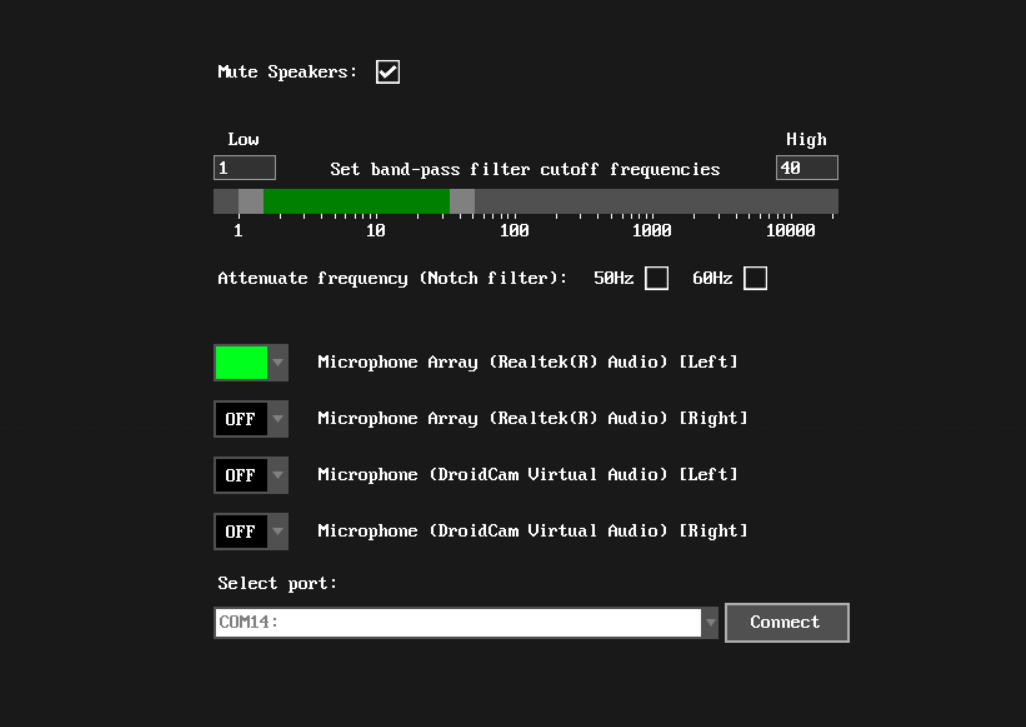
\includegraphics{images/clipboard-1531367267.png}

As soon as you start reading the EEG data it is very likely that you
will see something like the image given below. The waves here are too
large on the y axis and the filter that you set could most likely be
reset.

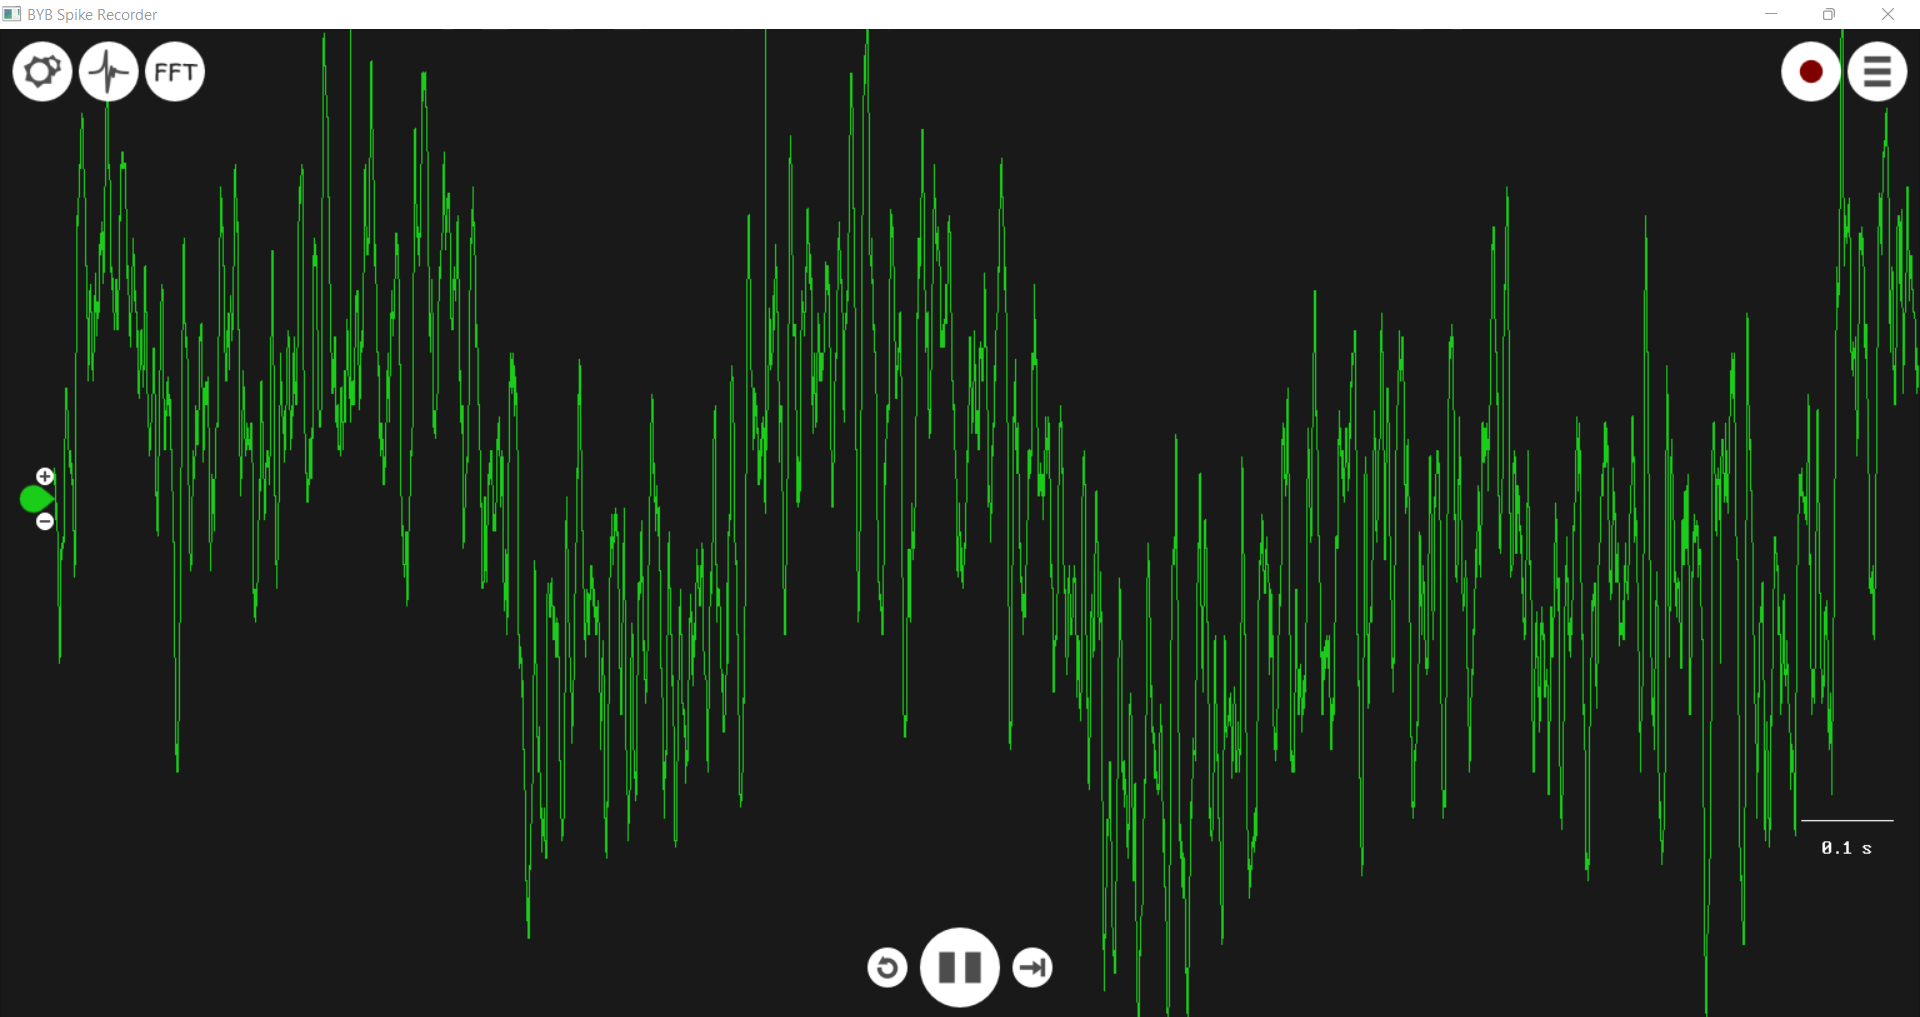
\includegraphics{images/clipboard-531262790.png}

There are two ways to fix this.

\begin{itemize}
\item
  Adjust the zoom level on the y axis using the + and - buttons. In this
  case, you will need to make it smaller
\item
  Reconfigure the bandpass filter between 1 to 40. Even if you did this
  step before, check if it has been implemented
\end{itemize}

Once these two steps are done, you wave should look something like this:

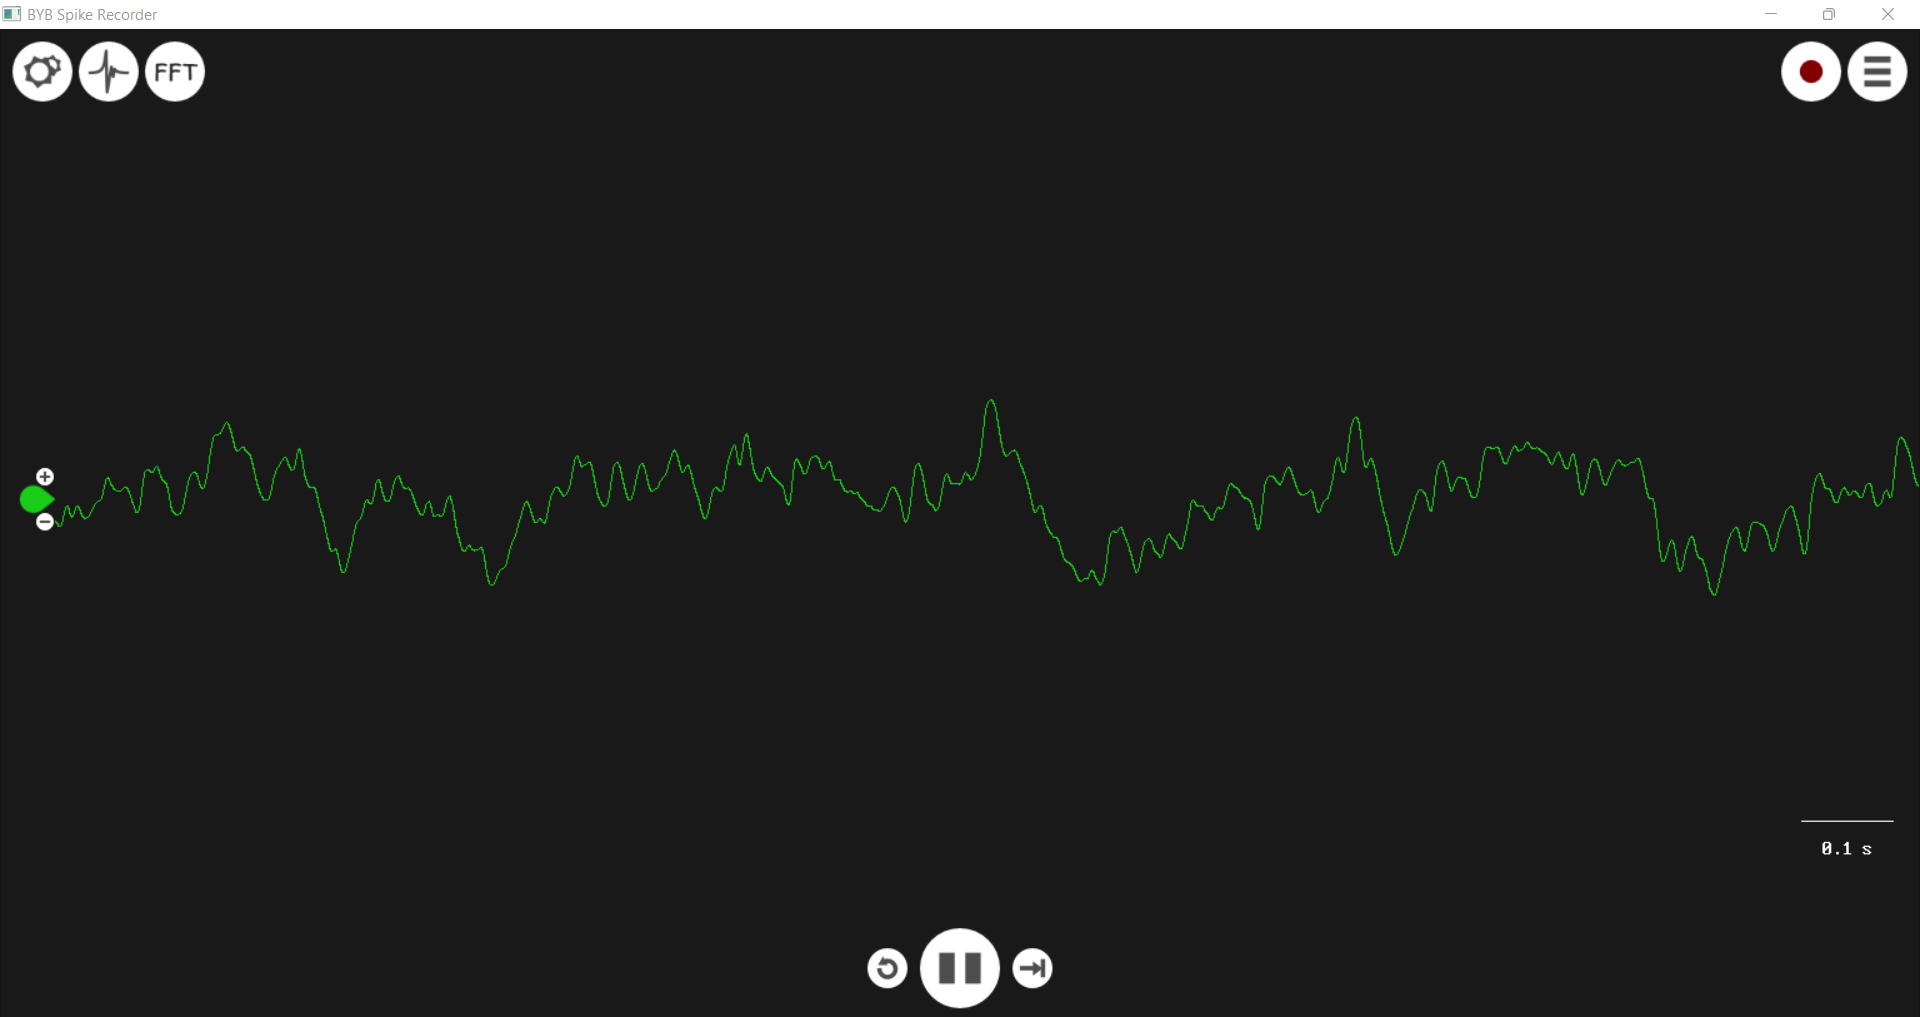
\includegraphics{images/clipboard-1600982436.png}

These are better representation of your EEG readings. To make sense of
brain activity and what is actually happening, we will need to use an
FFT graph. An FFT graph stands for Fast Fourier Transform graph and they
show which frequencies are present in a vibration during a certain
period of time. To enable the FFT graph click on the FFT button in the
top left corner.
